% 2017_shanghai_q12_fig1: grid 7x5 (35 squares) with P1-P4 dots and 4 triangle markers.
% Coordinates in cm; grid (0,0)-(7,5). Matches solution coords.
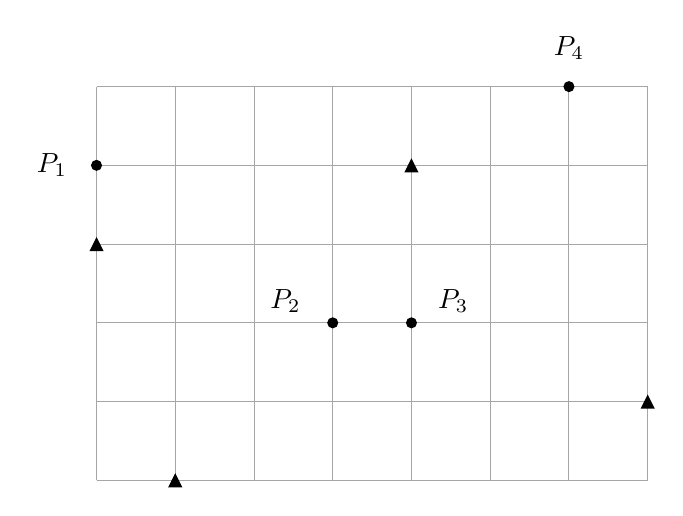
\begin{tikzpicture}[x=1cm,y=1cm,font=\normalsize,line width=.6pt]
\draw[draw=gray!70,line width=.35pt,step=1cm] (0,0) grid (7,5);
% triangle markers (filled small triangles, side ~0.22cm)
\foreach \p in {(1,0),(0,3),(4,4),(7,1)} {
  \fill[black] \p ++(0,0.09) -- ++(-0.09,-0.18) -- ++(0.18,0) -- cycle;
}
% dots P1-P4
\foreach \p in {(0,4),(3,2),(4,2),(6,5)} { \fill[black] \p circle (2pt); }
% labels with generous clearance (>=5pt from any stroke)
\node[anchor=east,xshift=-7pt] at (0,4) {$P_{1}$};
\node[anchor=east,xshift=-8pt,yshift=8pt] at (3,2) {$P_{2}$};
\node[anchor=west,xshift=6pt,yshift=8pt] at (4,2) {$P_{3}$};
\node[anchor=south,yshift=6pt] at (6,5) {$P_{4}$};
\end{tikzpicture}
